\documentclass{article}
\usepackage{geometry}
\usepackage{graphicx}
\usepackage{amsmath}
\usepackage{algorithm}
\usepackage{algpseudocode}
\usepackage{dsfont}
\usepackage{amssymb}
\usepackage{multicol}
\usepackage{wrapfig}
\usepackage{tipa}
\geometry{
a4paper,
right=10mm,
left=10mm,
top=10mm,
bottom=10mm,	
}

\begin{document}

\pagenumbering{gobble}

\begin{center}
\textbf{\Large HOMEWORK 3 : CS771} \\
\textit{\large Jayant Agrawal}         14282
\end{center}
\section{Problem 1- Kernel Perceptron}
\begin{figure}[h!]
\centering
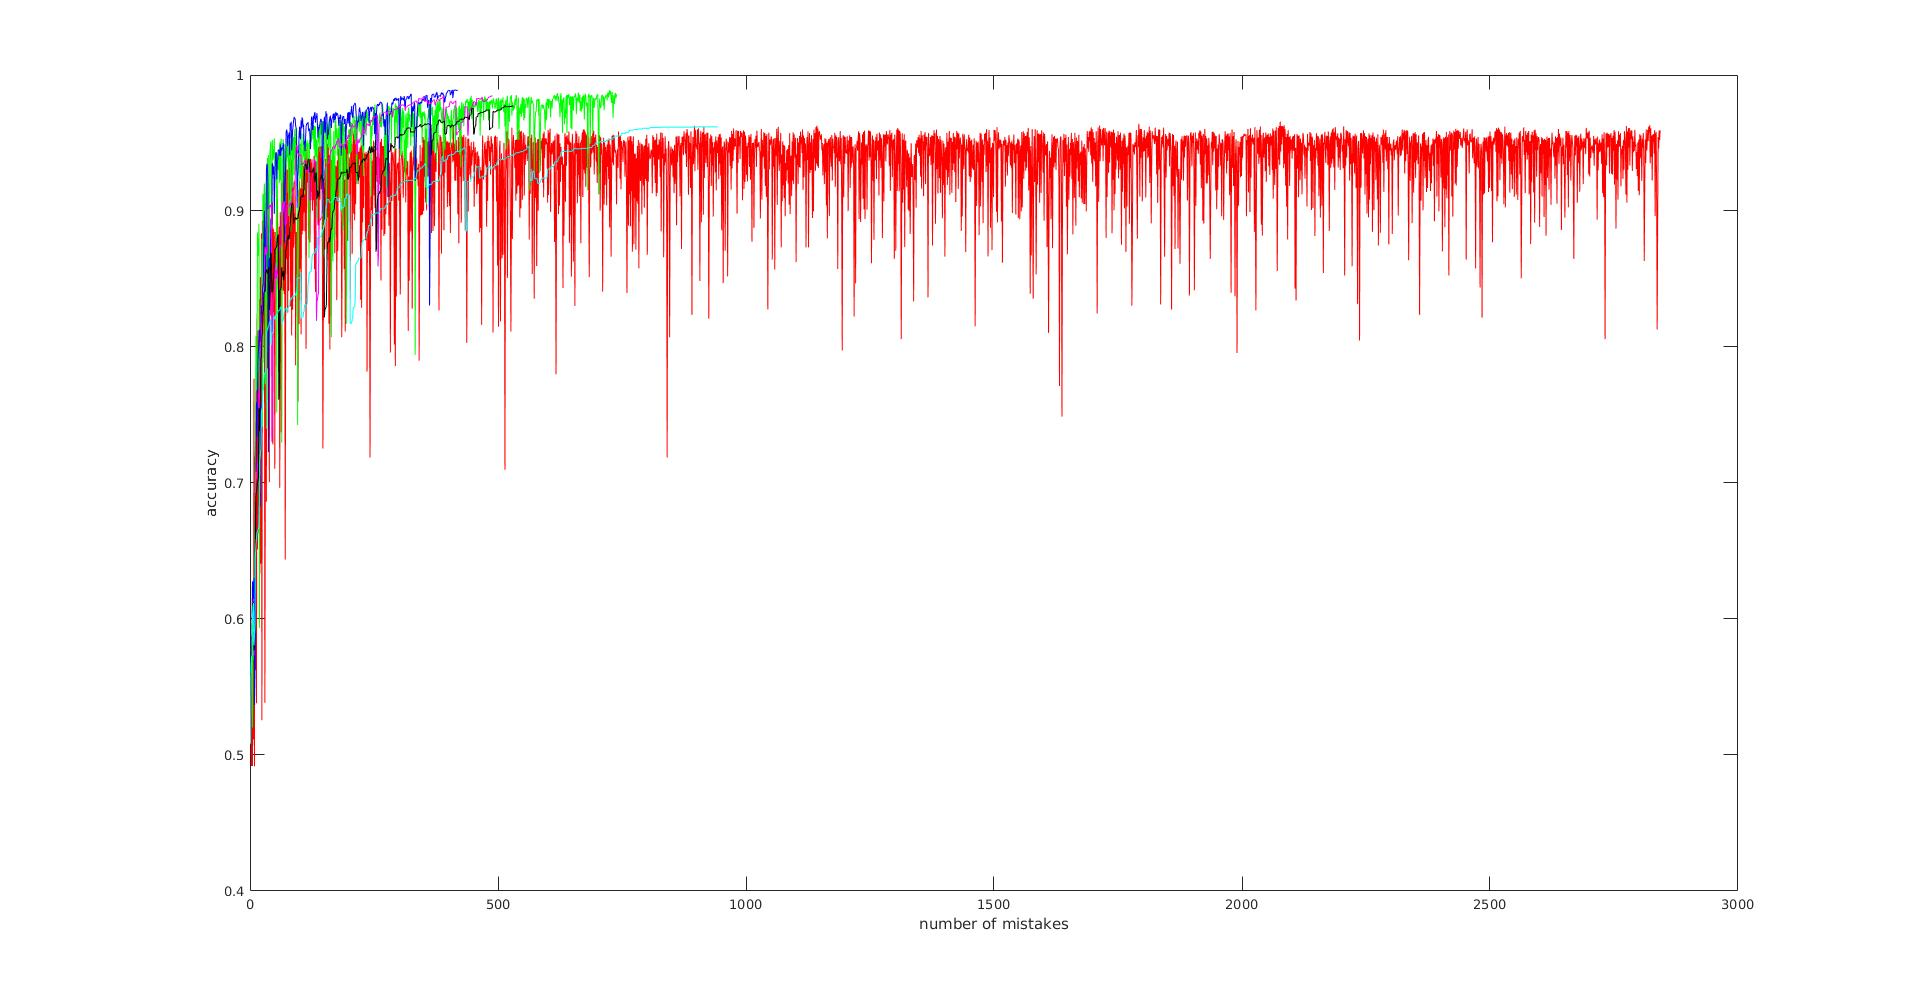
\includegraphics[width=1\columnwidth]{plot_acc.jpg}
\caption{Red = 1, Green = 2, Blue = 4, Pink = 8, Black = 10, Cyan = 20}
\label{acc}
\end{figure}
\begin{center}
\emph{Kernel with Test Accuracy: }4 (Blue)\\ 
\emph{Kernel with Minimum Mistakes: }4 (Blue) 
\end{center}

\section{Problem 2- Matrix Factorization}
\begin{figure}[h!]
\centering
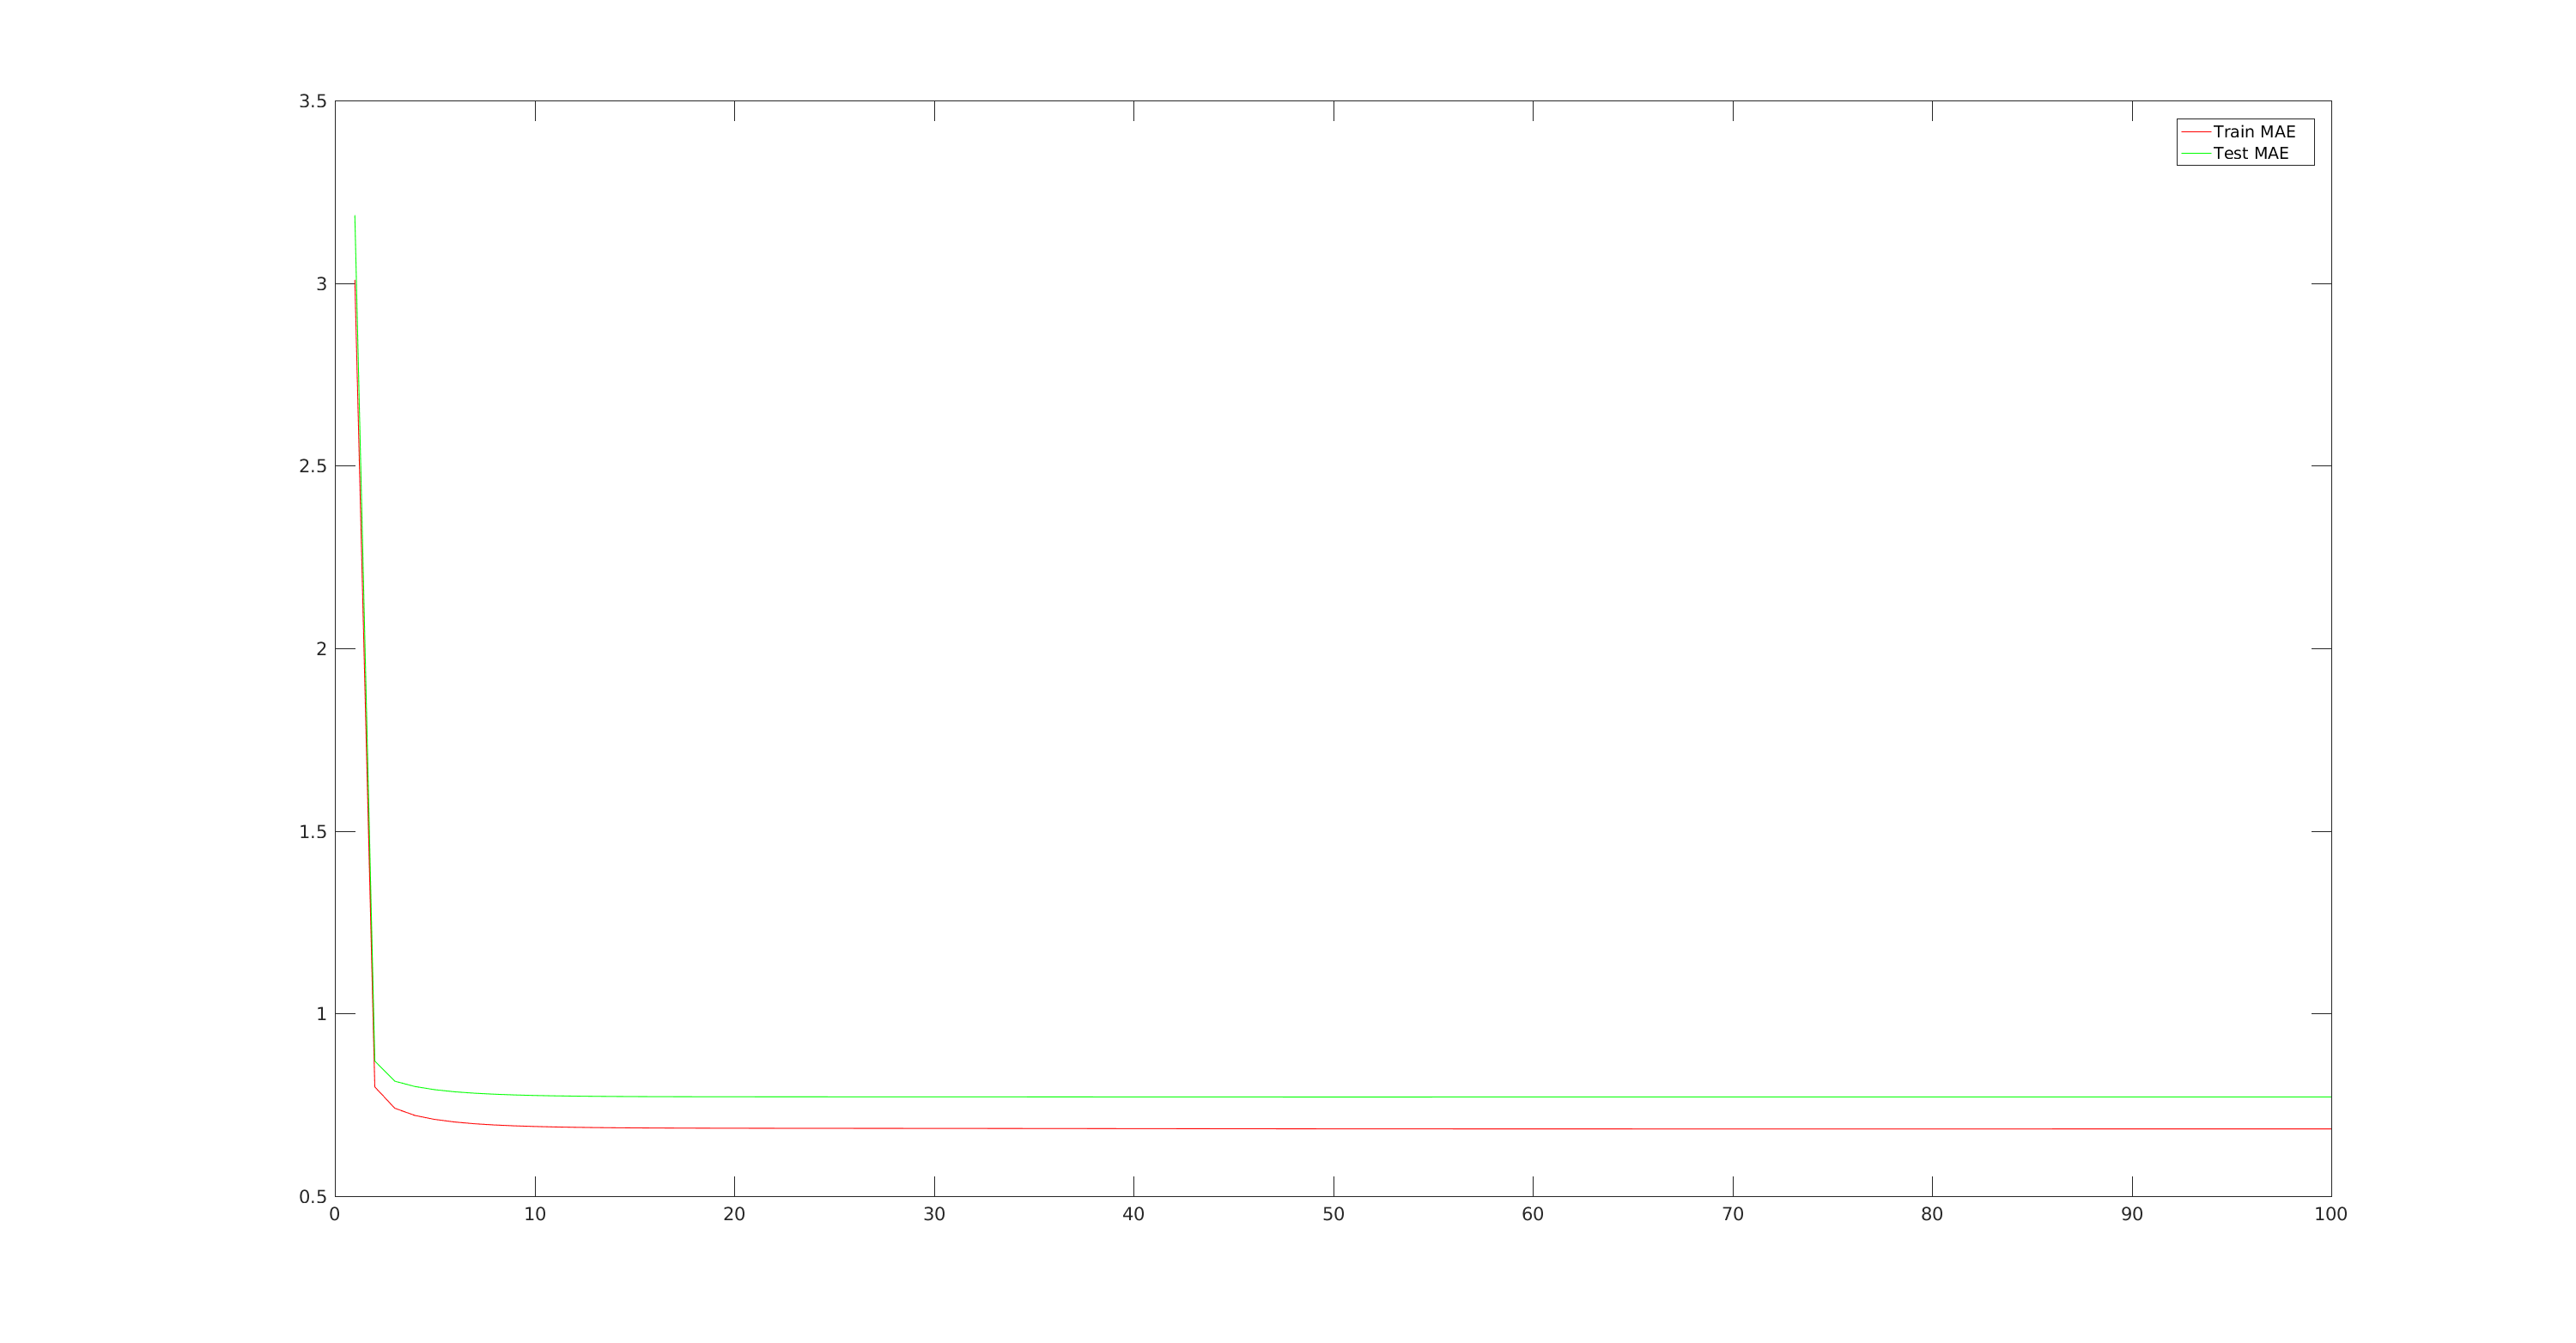
\includegraphics[width=1\columnwidth]{mae2.png}
%\caption{Red = 1, Green = 2, Blue = 4, Pink = 8, Black = 10, Cyan = 20}
\label{mae}
\end{figure}

\section{Problem 3 - GMM }
Assuming that gaussians have a shared spherical diagonal covariance matrix $\sigma^2\text{\textbf{I}}_D$.  Section \ref{sig} contains derivation for $\sigma^2$.
\subsection{Expression for $\sigma^2$}
\label{sig}
Expected Complete data Log-Likelihood ($\mathcal{L}$) for this model can be written as:
$$\mathcal{L} = \sum_{n=1}^N \sum_{k=1}^K \mathds{E}[z_{nk}][log\pi_k + log \mathcal{N}(x_n | \mu_k, \Sigma))]$$
where $\mathds{E}[z_{nk}] = \frac{\pi_k \mathcal{N}(x_n| \mu_k, \Sigma)}{\sum_{l=1}^K \mathcal{N}(x_n| \mu_k, \Sigma)}$ and $\Sigma = \sigma^2\textbf{I}_D$. Also, $\sum_{k=1}^K \mathds{E}[z_{nk}]=1$. \\ \\
Using $\mathds{E}[z_{nk}] = \gamma_{nk}$, taking derivative w.r.t $\mu_k$ and setting it to zero $\forall k = 1,...K $(The derivation for $u_k$ is similar to the general case shown in class except that $\Sigma_k$ is replaced by $\Sigma$), we get :
$$ \frac{\partial \mathcal{L}}{\partial \mu_k} = \frac{\partial}{\partial \mu_k} \sum_{n=1}^N \gamma_{nk} log \mathcal{N}(x_n | \mu_k, \Sigma) = 0 $$
We get the following expression for $\mu_k$, as shown in the note and lectures:
$$\mu_k = \frac{1}{N_k}\sum_{n=1}^N \gamma_{nk}x_n$$
where $N_k = \sum_{n=1}^N \gamma_{nk}$. \\ \\
Now, taking derivative of $\mathcal{L}$ w.r.t $\Sigma$:
\begin{equation*}
\begin{aligned}
\frac{\partial \mathcal{L}}{\partial \Sigma} &= \frac{\partial}{\partial \Sigma} \sum_{n=1}^N \sum_{k=1}^K \gamma_{nk}[ log \pi_k + log \mathcal{N}(x_n | \mu_k, \Sigma)] \\
&= \sum_{n=1}^N \sum_{k=1}^K \gamma_{nk} \frac{\partial}{\partial \Sigma} log \mathcal{N}(x_n | \mu_k, \Sigma) \\
\end{aligned}
\end{equation*}
Now, proceeding as shown in the note, Consider $log \mathcal{N}(x_n | \mu_k, \Sigma)$ :
\begin{equation*}
\begin{aligned}
log \mathcal{N}(x_n | \mu_k, \Sigma) &\propto - \frac{1}{2}log|\Sigma| - \frac{1}{2}(x_n- \mu_k)^T\Sigma^{-1}(x_n-\mu_k)\\
&= \frac{1}{2}log|\Sigma^{-1}| - \frac{1}{2}(x_n- \mu_k)^T\Sigma^{-1}(x_n-\mu_k) \\
&= \frac{1}{2}log|\Sigma^{-1}| - \frac{1}{2}tr[(x_n- \mu_k)(x_n-\mu_k)^T\Sigma^{-1} ]\\
\end{aligned}
\end{equation*}
Taking derivatives wrt. $\Sigma^{-1}$ (instead of $\Sigma$):
\begin{equation*}
\begin{aligned}
\sum_{n=1}^N\sum_{k=1}^K \gamma_{nk}\frac{\partial}{\partial \Sigma^{-1}}[ \frac{1}{2}log|\Sigma^{-1}| - \frac{1}{2}tr[(x_n- \mu_k)(x_n-\mu_k)^T\Sigma^{-1}]] &= 0\\
\sum_{n=1}^N\sum_{k=1}^K \gamma_{nk} [\Sigma - (x_n- \mu_k)(x_n-\mu_k)^T ] &=0 \\
\end{aligned}
\end{equation*}
Thus, we get the following expression for $\Sigma = \sigma^2\textbf{I}$:
\begin{equation*}
\begin{aligned}
\Sigma &= \frac{1}{\sum_{n=1}^N\sum_{k=1}^K \gamma_{nk}} \sum_{n=1}^N\sum_{k=1}^K \gamma_{nk}(x_n- \mu_k)(x_n-\mu_k)^T \\
\end{aligned}
\end{equation*}
Comparing the diagonal entries from the two sides, we get:
$$\sigma^2 = \frac{\sum_{n=1}^N (x_n^Tx_n - \sum_{k=1}^K \gamma_{nk}\mu_k^T\mu_k)}{\sum_{n=1}^N\sum_{k=1}^K \gamma_{nk}}$$
\section{Problem 4}
\section{Problem 5}
\end{document}


